\documentclass[a4paper, 11pt]{article}
%
\usepackage[utf8]{inputenc}
\usepackage[T1]{fontenc}
\usepackage{lmodern}
\usepackage[francais]{babel}
\usepackage[top=1cm, bottom=1cm, left=1cm, right=2cm]{geometry}
\usepackage{nopageno}
\usepackage{graphicx}
%
\newcommand{\env}[1]{\fbox{\begin{minipage}{\textwidth}#1\end{minipage}}}
%
\title{Exo SD 2 Points}
\author{Sarfraz \bsc{kapasi}}
\date{14/02/2013}
%
\begin{document}
%
\maketitle
%
\section{Conversion de doublets en représentation à points}

Reprenez les schémas à doublet de la première partie des exercices sur la représentation interne des listes et donnez leur représentation à points\\

\begin{enumerate}
  \item 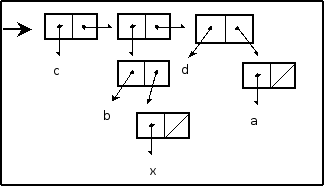
\includegraphics[height=120pt, width=180pt]{Pointeurs_Exo1.png}\\
Réponse: (c . ((b . (x . nil)) . (d . (a . nil))))
  \item 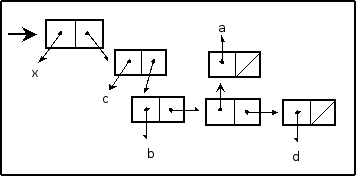
\includegraphics[height=120pt, width=180pt]{Pointeurs_Exo2.png}\\
Réponse: (x . (c . (b . ((a . nil) . (d . nil)))))
  \item 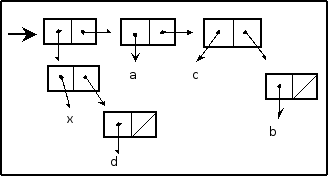
\includegraphics[height=120pt, width=180pt]{Pointeurs_Exo3.png}\\
Réponse: ((x . (d . nil)) . (a . (c . (b . nil))))
  \item 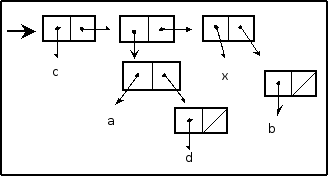
\includegraphics[height=120pt, width=180pt]{Pointeurs_Exo4.png}\\
Réponse: (c . ((a . (d . nil)) . (x . (b . nil))))
  \item 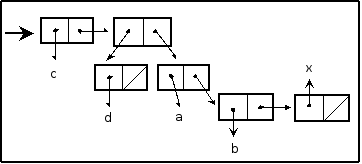
\includegraphics[height=120pt, width=180pt]{Pointeurs_Exo5.png}\\
Réponse: (c . ((d . nil) . (a . (b . (x . nil)))))
  \item 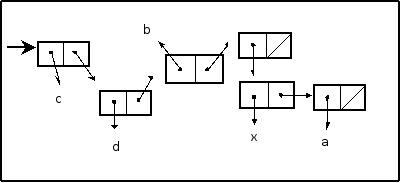
\includegraphics[height=120pt, width=180pt]{Pointeurs_Exo6.png}\\
Réponse: (c . (d . (b . ((x . (a . nil)) . nil))))
\end{enumerate}

\section{Conversion de représentation à points en doublets}

 Donnez (avec Dia) la représentation en doublets de pointeurs des exemples suivants:\\

\begin{enumerate}
    \item (a . ((b . c) . (x . nil)))\\ 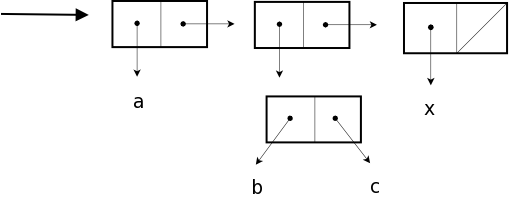
\includegraphics[scale=0.3]{reponse1.png}
    \item ((a . nil) . ((b . (c . nil)) . nil))\\ 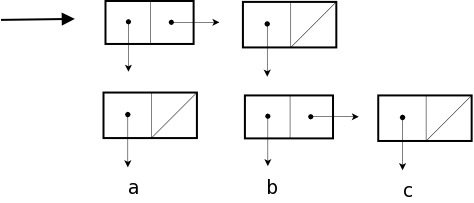
\includegraphics[scale=0.3]{reponse2.png}
    \item ((a . (b . nil)) . (d . (c . nil)))\\ 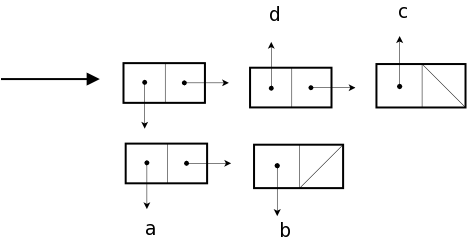
\includegraphics[scale=0.3]{reponse3.png}
    \item (a . (b . (c . (d . nil))))\\ 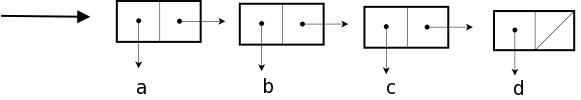
\includegraphics[scale=0.3]{reponse4.png}
    \item (a . ((b . nil) . (d . (c . nil))))\\ 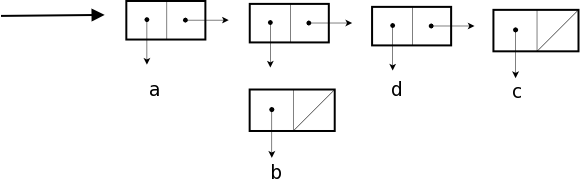
\includegraphics[scale=0.3]{reponse5.png}
    \item (a . (c . d . ((b . e) . nil)))\\ 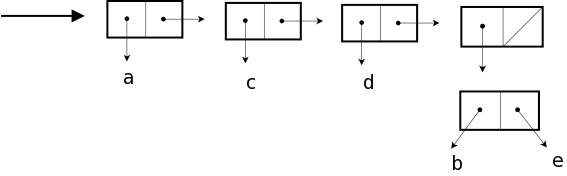
\includegraphics[scale=0.3]{reponse6.png}
\end{enumerate}
%
\end{document}
